% Options for packages loaded elsewhere
\PassOptionsToPackage{unicode}{hyperref}
\PassOptionsToPackage{hyphens}{url}
\PassOptionsToPackage{dvipsnames,svgnames,x11names}{xcolor}
%
\documentclass[
  letterpaper,
  DIV=11,
  numbers=noendperiod]{scrartcl}
\usepackage{beamerarticle} % needs to be loaded first

\usepackage{amsmath,amssymb}
\usepackage{iftex}
\ifPDFTeX
  \usepackage[T1]{fontenc}
  \usepackage[utf8]{inputenc}
  \usepackage{textcomp} % provide euro and other symbols
\else % if luatex or xetex
  \usepackage{unicode-math}
  \defaultfontfeatures{Scale=MatchLowercase}
  \defaultfontfeatures[\rmfamily]{Ligatures=TeX,Scale=1}
\fi
\usepackage{lmodern}
\ifPDFTeX\else  
    % xetex/luatex font selection
\fi
% Use upquote if available, for straight quotes in verbatim environments
\IfFileExists{upquote.sty}{\usepackage{upquote}}{}
\IfFileExists{microtype.sty}{% use microtype if available
  \usepackage[]{microtype}
  \UseMicrotypeSet[protrusion]{basicmath} % disable protrusion for tt fonts
}{}
\makeatletter
\@ifundefined{KOMAClassName}{% if non-KOMA class
  \IfFileExists{parskip.sty}{%
    \usepackage{parskip}
  }{% else
    \setlength{\parindent}{0pt}
    \setlength{\parskip}{6pt plus 2pt minus 1pt}}
}{% if KOMA class
  \KOMAoptions{parskip=half}}
\makeatother
\usepackage{xcolor}
\setlength{\emergencystretch}{3em} % prevent overfull lines
\setcounter{secnumdepth}{5}
% Make \paragraph and \subparagraph free-standing
\ifx\paragraph\undefined\else
  \let\oldparagraph\paragraph
  \renewcommand{\paragraph}[1]{\oldparagraph{#1}\mbox{}}
\fi
\ifx\subparagraph\undefined\else
  \let\oldsubparagraph\subparagraph
  \renewcommand{\subparagraph}[1]{\oldsubparagraph{#1}\mbox{}}
\fi


\providecommand{\tightlist}{%
  \setlength{\itemsep}{0pt}\setlength{\parskip}{0pt}}\usepackage{longtable,booktabs,array}
\usepackage{calc} % for calculating minipage widths
% Correct order of tables after \paragraph or \subparagraph
\usepackage{etoolbox}
\makeatletter
\patchcmd\longtable{\par}{\if@noskipsec\mbox{}\fi\par}{}{}
\makeatother
% Allow footnotes in longtable head/foot
\IfFileExists{footnotehyper.sty}{\usepackage{footnotehyper}}{\usepackage{footnote}}
\makesavenoteenv{longtable}
\usepackage{graphicx}
\makeatletter
\def\maxwidth{\ifdim\Gin@nat@width>\linewidth\linewidth\else\Gin@nat@width\fi}
\def\maxheight{\ifdim\Gin@nat@height>\textheight\textheight\else\Gin@nat@height\fi}
\makeatother
% Scale images if necessary, so that they will not overflow the page
% margins by default, and it is still possible to overwrite the defaults
% using explicit options in \includegraphics[width, height, ...]{}
\setkeys{Gin}{width=\maxwidth,height=\maxheight,keepaspectratio}
% Set default figure placement to htbp
\makeatletter
\def\fps@figure{htbp}
\makeatother

\KOMAoption{captions}{tableheading}
\makeatletter
\@ifpackageloaded{caption}{}{\usepackage{caption}}
\AtBeginDocument{%
\ifdefined\contentsname
  \renewcommand*\contentsname{Table of contents}
\else
  \newcommand\contentsname{Table of contents}
\fi
\ifdefined\listfigurename
  \renewcommand*\listfigurename{List of Figures}
\else
  \newcommand\listfigurename{List of Figures}
\fi
\ifdefined\listtablename
  \renewcommand*\listtablename{List of Tables}
\else
  \newcommand\listtablename{List of Tables}
\fi
\ifdefined\figurename
  \renewcommand*\figurename{Figure}
\else
  \newcommand\figurename{Figure}
\fi
\ifdefined\tablename
  \renewcommand*\tablename{Table}
\else
  \newcommand\tablename{Table}
\fi
}
\@ifpackageloaded{float}{}{\usepackage{float}}
\floatstyle{ruled}
\@ifundefined{c@chapter}{\newfloat{codelisting}{h}{lop}}{\newfloat{codelisting}{h}{lop}[chapter]}
\floatname{codelisting}{Listing}
\newcommand*\listoflistings{\listof{codelisting}{List of Listings}}
\makeatother
\makeatletter
\makeatother
\makeatletter
\@ifpackageloaded{caption}{}{\usepackage{caption}}
\@ifpackageloaded{subcaption}{}{\usepackage{subcaption}}
\makeatother
\ifLuaTeX
  \usepackage{selnolig}  % disable illegal ligatures
\fi
\usepackage{bookmark}

\IfFileExists{xurl.sty}{\usepackage{xurl}}{} % add URL line breaks if available
\urlstyle{same} % disable monospaced font for URLs
\hypersetup{
  pdftitle={Technology enabled mathematical science education},
  pdfauthor={Emma Cliffe},
  colorlinks=true,
  linkcolor={blue},
  filecolor={Maroon},
  citecolor={Blue},
  urlcolor={Blue},
  pdfcreator={LaTeX via pandoc}}

\title{Technology \emph{enabled} mathematical science education}
\usepackage{etoolbox}
\makeatletter
\providecommand{\subtitle}[1]{% add subtitle to \maketitle
  \apptocmd{\@title}{\par {\large #1 \par}}{}{}
}
\makeatother
\subtitle{Bridging Research and Practice}
\author{Emma Cliffe}
\date{}

\begin{document}
\maketitle

\renewcommand*\contentsname{Table of contents}
{
\hypersetup{linkcolor=}
\setcounter{tocdepth}{3}
\tableofcontents
}
\textbf{Abstract}: This talk will explore key research and technological
developments that have enabled access to mathematical resources for all
students, including disabled students. We will examine the role of
specialist practitioners in translating research and development outputs
into practical methods for the average mathematics lecturer,
contributing to changes in everyday practices. We will review remaining
core technical access issues and discuss how our community can
effectively respond to these challenges, using two specific examples to
guide our conversation.

\section{Enabling access}\label{enabling-access}

\subsection{Defining the problem}\label{defining-the-problem-1}

\subsubsection{We want\ldots{}}\label{we-want}

\ldots{} to enable access to mathematical content by:

\begin{itemize}
\tightlist
\item
  People using assistive technology
\item
  People reading on small screen devices, e-book readers\ldots{}
\item
  People searching, copying and pasting
\item
  People verifying reproducibility of results
\item
  Software parsing, transforming, generating and manipulating input and
  output
\item
  AIs consuming and generating mathematical content\ldots?
\end{itemize}

\subsubsection{\texorpdfstring{\href{./quadratic.pdf}{But\ldots{}}}{But\ldots{}}}\label{but}

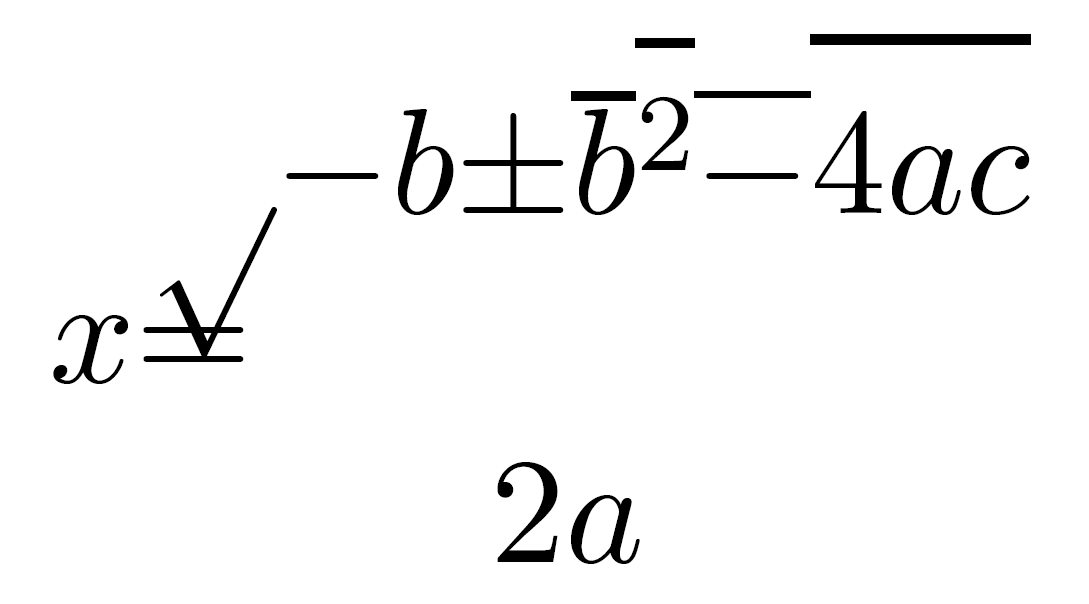
\includegraphics{./images/reflowing.png}\\

\subsubsection{\texorpdfstring{\href{./images/alt/Legal-context.xlsx}{Legal}}{Legal}}\label{legal}

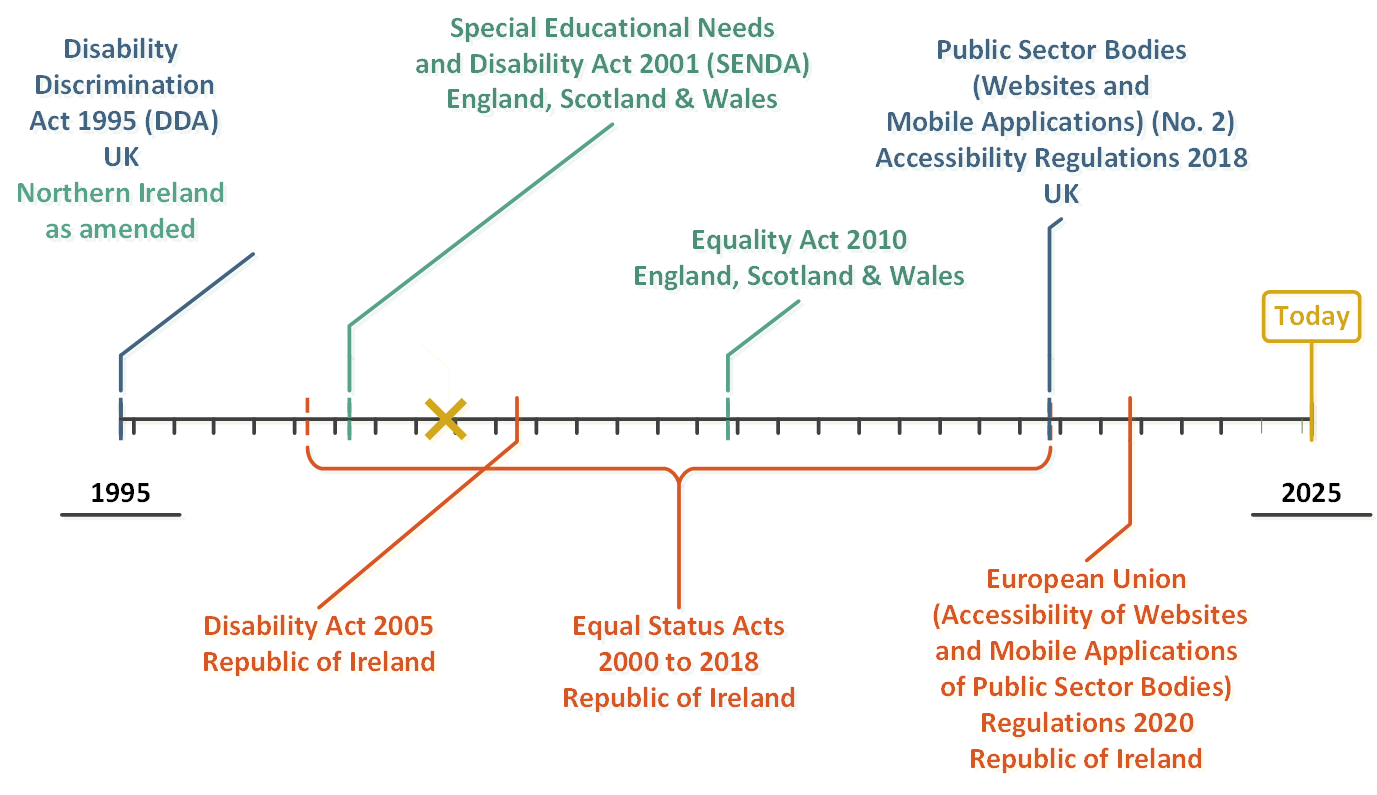
\includegraphics{./images/Legal-context.png}\\

\subsection{From research to practice}\label{from-research-to-practice}

\subsubsection{\texorpdfstring{\href{./images/alt/Technology-context.xlsx}{Technical}}{Technical}}\label{technical}

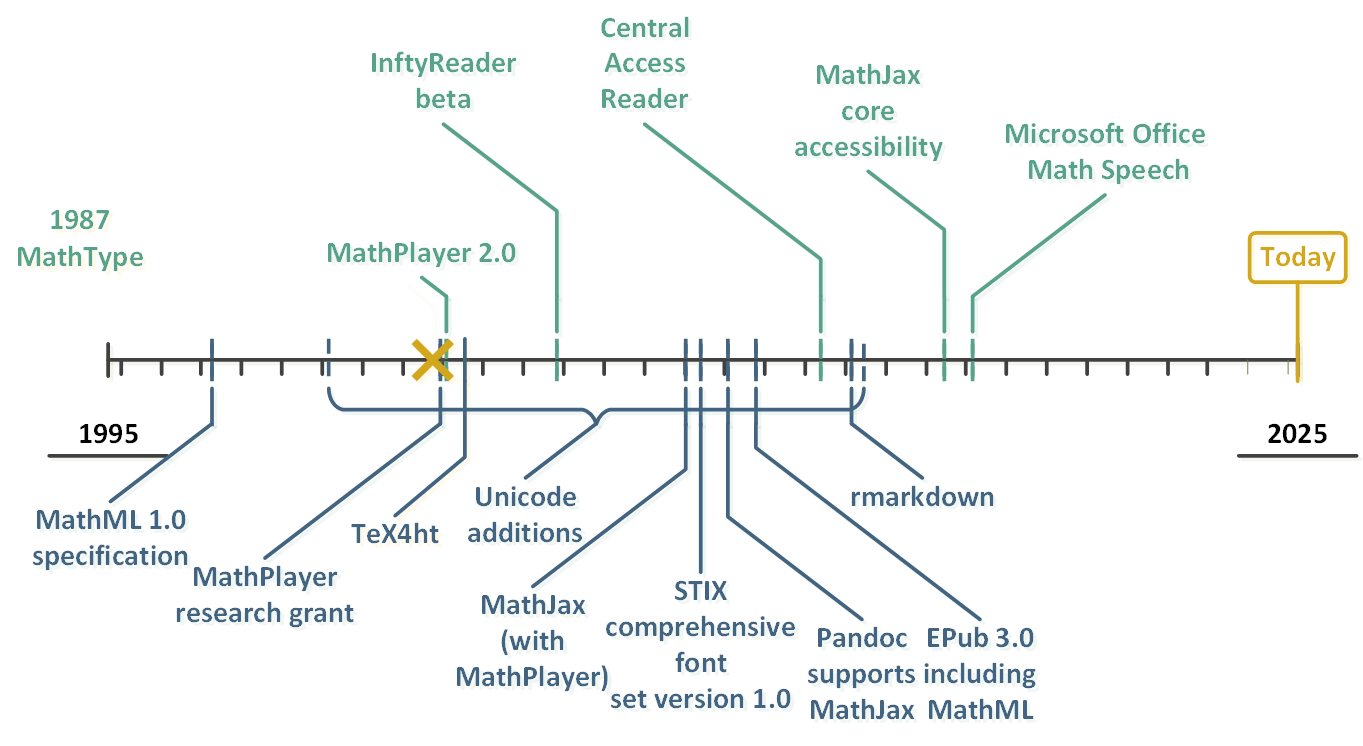
\includegraphics{./images/Technology-context.png}\\

\subsubsection{\texorpdfstring{\href{./images/alt/Our-work.xlsx}{Practitioners}}{Practitioners}}\label{practitioners}

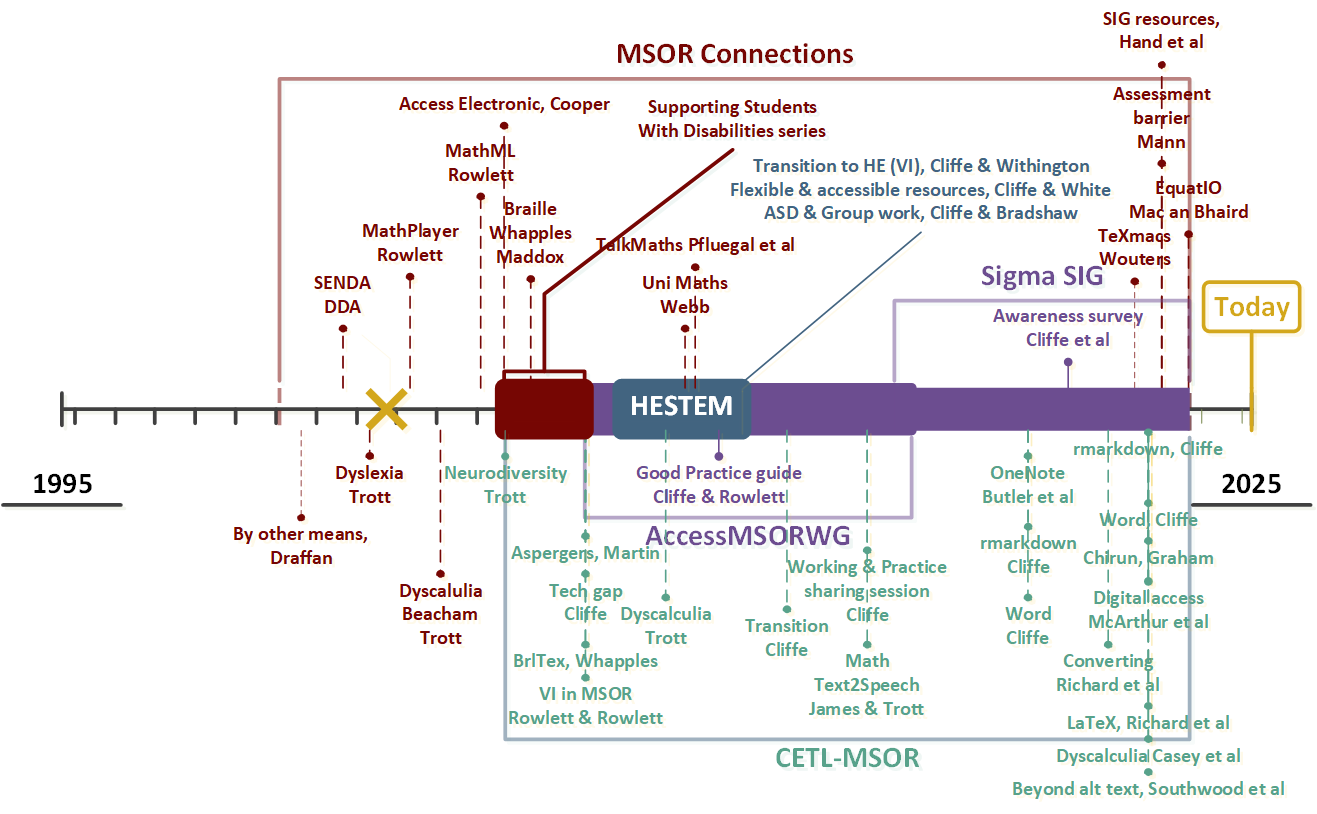
\includegraphics{./images/Our-work.png}\\

\subsubsection{\texorpdfstring{\href{./images/alt/Our-work-phases.xlsx}{Phases}}{Phases}}\label{phases}

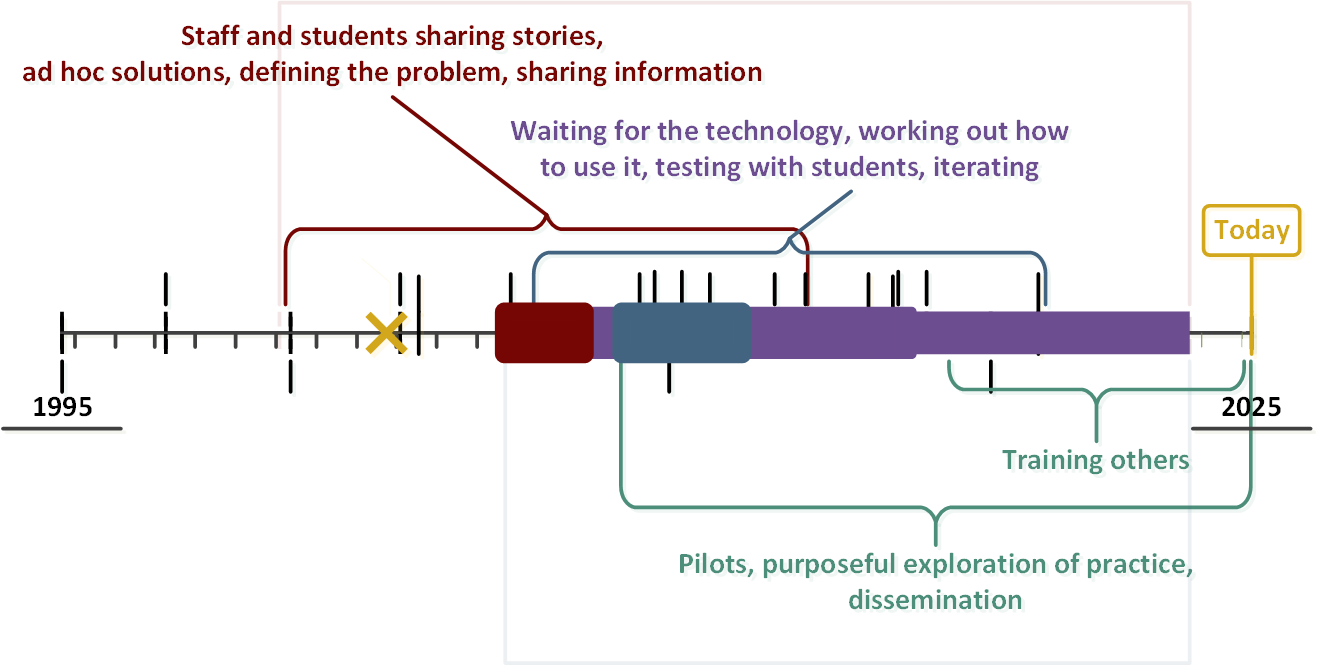
\includegraphics{./images/Our-work-phases.png}\\

\subsection{Change}\label{change}

\subsubsection{\texorpdfstring{\href{https://teachinghub.bath.ac.uk/guide-category/technical-accessibility/}{CLT
\& Lecturers}}{CLT \& Lecturers}}\label{clt-lecturers}


\includegraphics{./images/CLT.png}\\

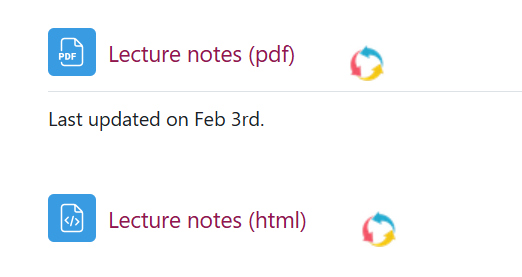
\includegraphics[width=0.65\textwidth,height=\textheight]{./images/notes.png}\\
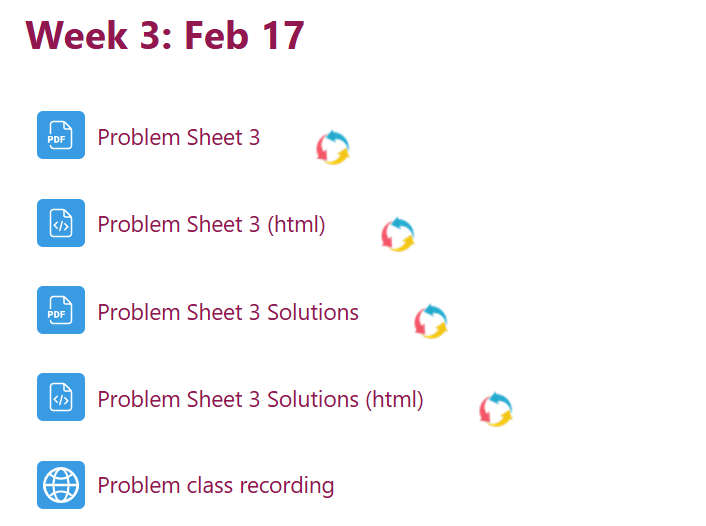
\includegraphics[width=0.8\textwidth,height=\textheight]{./images/sheets.png}\\

\subsubsection{\texorpdfstring{\href{./index.html\#mash-everyone}{MASH
\& Everyone!}}{MASH \& Everyone!}}\label{mash-everyone}

\paragraph{Maths support}\label{maths-support}


\includegraphics{./images/MASH.png}\\

\paragraph{MathJax}\label{mathjax}

\[
x = \frac{-b \pm \sqrt{b^2-4ac}}{2a}
\]

\paragraph{Desmos}\label{desmos}

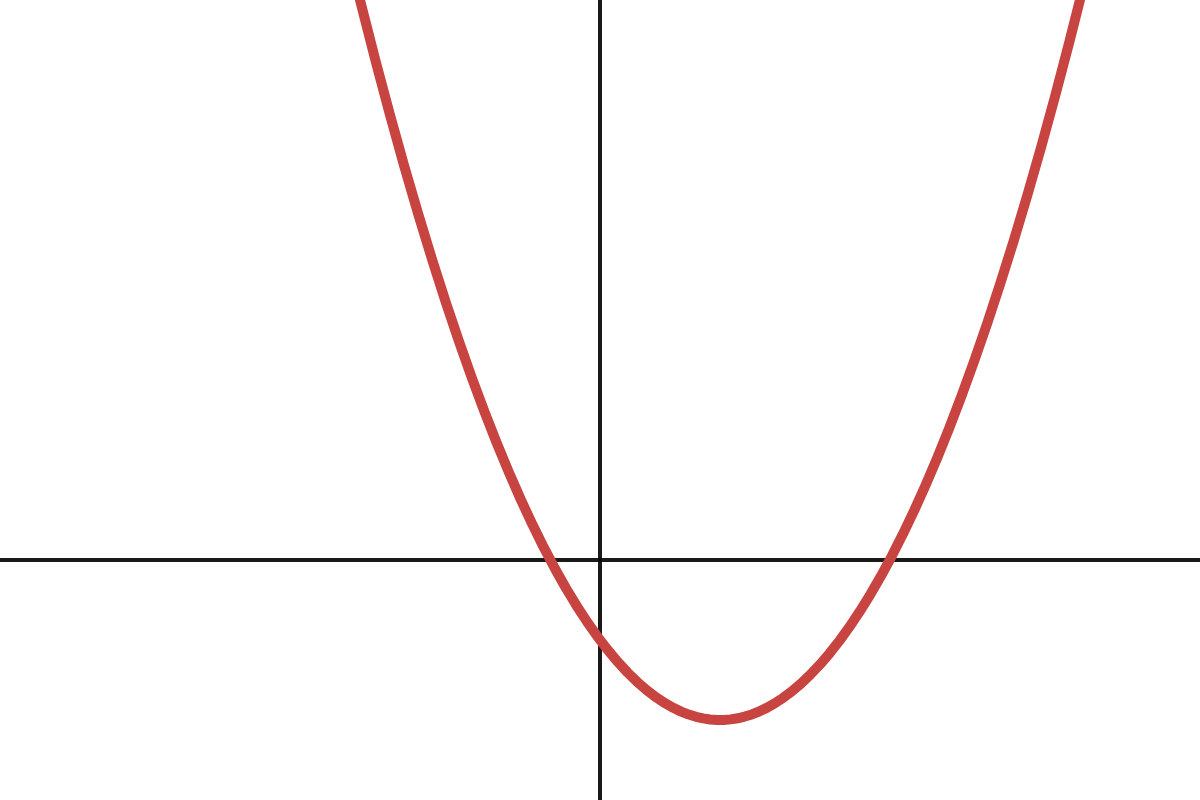
\includegraphics[width=0.8\textwidth,height=\textheight]{./images/desmos-quadratic.png}\\
\href{https://www.desmos.com/calculator/34qsxjk2p3}{Interactive
accessible version of the quadratic graph}

\section{What next?}\label{what-next}

\subsection{Dissemination and core
challenges}\label{dissemination-and-core-challenges}

\subsubsection{Getting started\ldots{}}\label{getting-started}

\begin{itemize}
\tightlist
\item
  \href{https://stem-enable.github.io/RMarkdownWorkshop/}{RMarkdown},
  \href{https://bookdown.org/}{Bookdown} and possibly
  \href{https://bathmash.github.io/clavertondown/}{ClavertonDown}
\item
  \href{https://quarto.org/}{Quarto}
\item
  \href{https://chirun.org.uk/}{Chirun}
\item
  \href{https://people.bath.ac.uk/feb/lwarp/lwarp-intro.html}{LWarp}
\item
  \href{https://pretextbook.org/}{PreTeXt}
\item
  \href{https://stem-enable.github.io/WordWorkshop/}{Word}
\item
  \href{https://bathmash.github.io/CETL-MSOR-2022-Beyond-alt-text/}{Desmos
  and Geogebra}
\item
  \href{https://r-resources.massey.ac.nz/BrailleR/}{BrailleR}
\end{itemize}

\subsubsection{Dissemination}\label{dissemination}

We are still doing this, now others are too\ldots{} Can you:

\begin{itemize}
\tightlist
\item
  Have a go yourself and tell others?
\item
  Join \href{https://github.com/A11yMaths}{JISC Accessibility Community
  Maths Working Group}
\item
  Consider and communicate regarding the implications for mathematical
  pedagogy?
\item
  Consider and communicate regarding the implications for open and
  reproducible science?
\item
  Build functionality into software and packages you create so that
  users automatically produce accessible output?
\end{itemize}

\subsubsection{Diagrams}\label{diagrams}

\begin{itemize}
\tightlist
\item
  It is possible to use Desmos, some functionality of Geogebra and the
  BrailleR package to help make accessible diagrams
\item
  This is nowhere near sufficient or flexible enough to represent the
  variety of diagrams we produce in e.g.~TikZ
\item
  These formats are not easily consumed and manipulated by other
  software or AIs
\end{itemize}

\subsubsection{Meaning}\label{meaning}

\begin{itemize}
\tightlist
\item
  We are no longer losing syntactic structure
\item
  We are still losing enough of the semantics \emph{known to the author}
  that things we want to do are affected

  \begin{itemize}
  \tightlist
  \item
    Sometimes the author encodes these in their LaTeX
  \item
    Not always though\ldots{}
  \end{itemize}
\item
  Consider \[
  \lvert\{(a,b) \mid a \in A, b \in B\}\rvert
  \]
\end{itemize}

\subsubsection{Questions and discussion}\label{questions-and-discussion}

Thank you for your time! Papers for discussion:

\begin{itemize}
\tightlist
\item
  \href{https://doi.org/10.1145/3587281.3587297}{Authoring
  Web-accessible Mathematical Diagrams.}
\item
  \href{https://doi.org/10.1007/978-3-031-62846-7_21}{Author Intent:
  Eliminating Ambiguity in MathML.},
  \href{https://arxiv.org/abs/2407.06720}{Pre-print}
\end{itemize}

Slides: \url{https://ehcliffe.github.io/TEMSE2025/}

My email address:
\href{mailto:E.H.Cliffe@bath.ac.uk}{\nolinkurl{E.H.Cliffe@bath.ac.uk}}

\begin{figure}

\begin{minipage}{0.50\linewidth}

\includegraphics[width=0.75\textwidth,height=\textheight]{./images/MASH-logo.png}\\
\end{minipage}%
%
\begin{minipage}{0.50\linewidth}

\includegraphics[width=0.6\textwidth,height=\textheight]{./images/uob-logo-grey-transparent.png}\\
\end{minipage}%

\end{figure}%



\end{document}
